% !TEX root = ../rasd.tex
\chapter{Alloy Modelling}
\label{alloy}

In this chapter the consistency of the UML class diagram will be tested using Alloy Analyzer. In the following paragraph there will be shown first the code used, then the response of Alloy, using assertions, predicates and an example of a possible world.

\section{Alloy Code}
Here the code used is presented.

\lstinputlisting[language=alloy]{./code/alloy/ALLOY_myTaxiService.als}

\clearpage

\section{Alloy Response}
Here the alloy response to the model is shown.
\begin{Verbatim}[commandchars=\\\{\},codes={\catcode`$=3\catcode`_=8}]
Executing "Check driversInTheQueue for 5 but exactly 3 Area, 2 FutureRide, exactly 3 Driver"
   Solver=sat4j Bitwidth=4 MaxSeq=5 SkolemDepth=1 Symmetry=20
   7123 vars. 454 primary vars. 15513 clauses. 369ms.
   Counterexample found. Assertion is invalid. 81ms.

Executing "Check multipleReservation for 5"
   Solver=sat4j Bitwidth=4 MaxSeq=5 SkolemDepth=1 Symmetry=20
   8431 vars. 541 primary vars. 18192 clauses. 320ms.
   Counterexample found. Assertion is invalid. 66ms.

Executing "Check noUbiquity for 5"
   Solver=sat4j Bitwidth=4 MaxSeq=5 SkolemDepth=1 Symmetry=20
   8976 vars. 536 primary vars. 19819 clauses. 242ms.
   No counterexample found. Assertion may be valid. 176ms.

Executing "Run noDriverAsCustomer for 5"
   Solver=sat4j Bitwidth=4 MaxSeq=5 SkolemDepth=1 Symmetry=20
   8437 vars. 526 primary vars. 18365 clauses. 180ms.
   Instance found. Predicate is consistent. 89ms.

Executing "Run show for 4"
   Solver=sat4j Bitwidth=4 MaxSeq=4 SkolemDepth=1 Symmetry=20
   5807 vars. 376 primary vars. 12745 clauses. 134ms.
   Instance found. Predicate is consistent. 72ms.

5 commands were executed. The results are:
   #1: Counterexample found. driversInTheQueue is invalid.
   #2: Counterexample found. multipleReservation is invalid.
   #3: No counterexample found. noUbiquity may be valid.
   #4: \textbf{Instance found}. noDriverAsCustomer is consistent.
   #5: \textbf{Instance found}. show is consistent.
\end{Verbatim}

\subsection{Counterexamples}
Two of the assertions we wrote are, in our idea, wrong assertions for the following reasons: the first one shows the correctness of a property of the model (a driver can be into a queue only when is waiting for a ride), the second one use the counterexample to proof the validity of another model property (an user that is traveling on a zerotime ride can book a future ride). In fact for the latter one there is no way to write the opposite assertion.

\label{cex1}
\begin{figure}[h!]
	\centerline{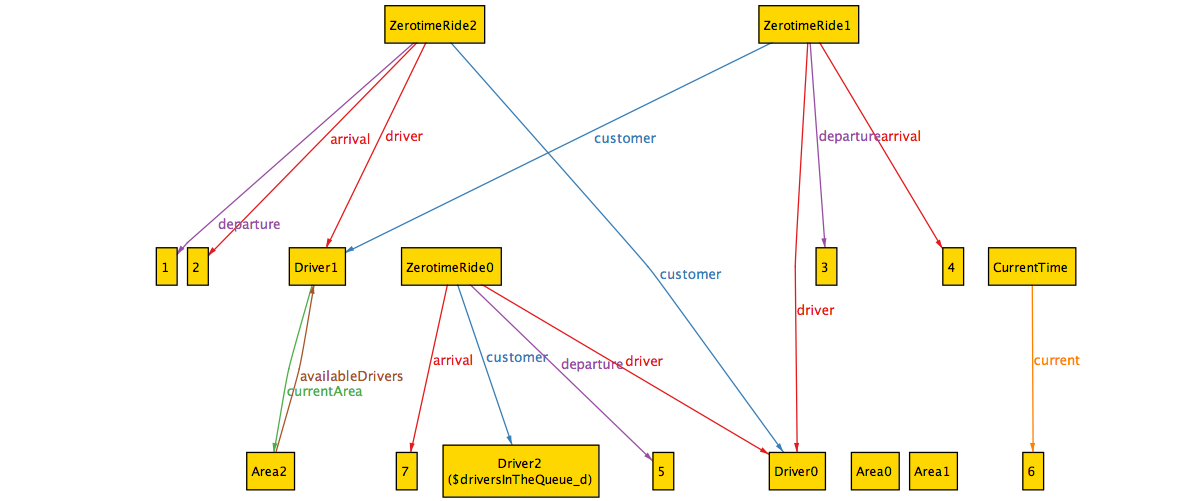
\includegraphics[width=\textheight, angle=90]{./figures/ALLOY_FirstAssertionCounterexample.png}}
	\caption{First Counterexample representation.\\
			\textbf{Note}: It is immediately visible that Driver1 is the driver assigned to ZerotimeRide2 and he is inserted into the Area2 queue. This is possible because the ride has already finished, so according to the model the driver must be waiting for another ride.}
	\label{cex1fig}
\end{figure}

\clearpage

\label{cex2}
\begin{figure}[h!]
	\centerline{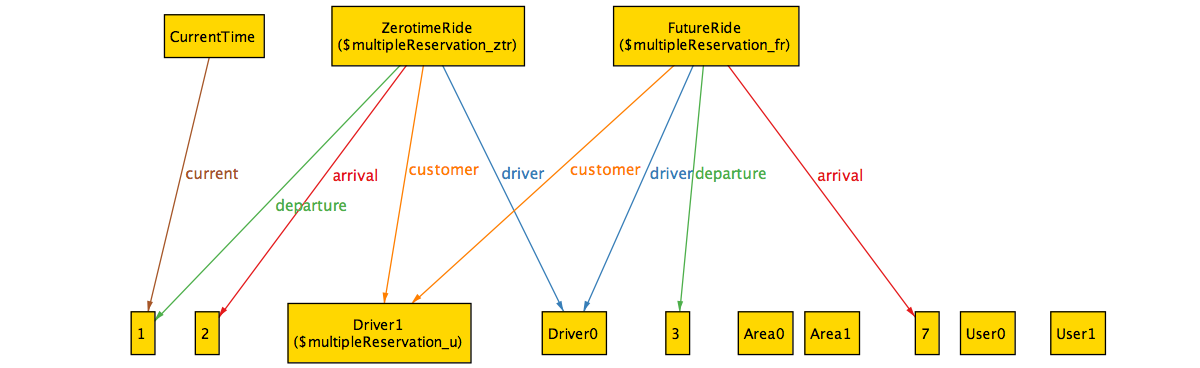
\includegraphics[width=\textheight, angle=90]{./figures/ALLOY_SecondAssertionCounterexample.png}}
	\caption{Second Counterexample representation}
	\label{cex2fig}
\end{figure}

\clearpage

\subsection{Alloy World}
In this paragraph are showed two worlds.\\
The former one shows a "restricted" world where only the users can be a customer. In the latter one the strange case of a driver who is traveling as customer in an other ride is allowed. Besides, the positions are shown to give a more complete and precise idea of the world.\\
\\
In all the images, the classes which are defined only in the Alloy model are hidden in order to have a clearer images. The unicity of email and taxCode of each User and the unicity of cab carCode are correctly defined into the model, but they are not as so important as the kinds of the rides and the management of the areas and the queues.

\clearpage

\subsubsection{World 1}
\label{w1}
\begin{figure}[h!]
	\centerline{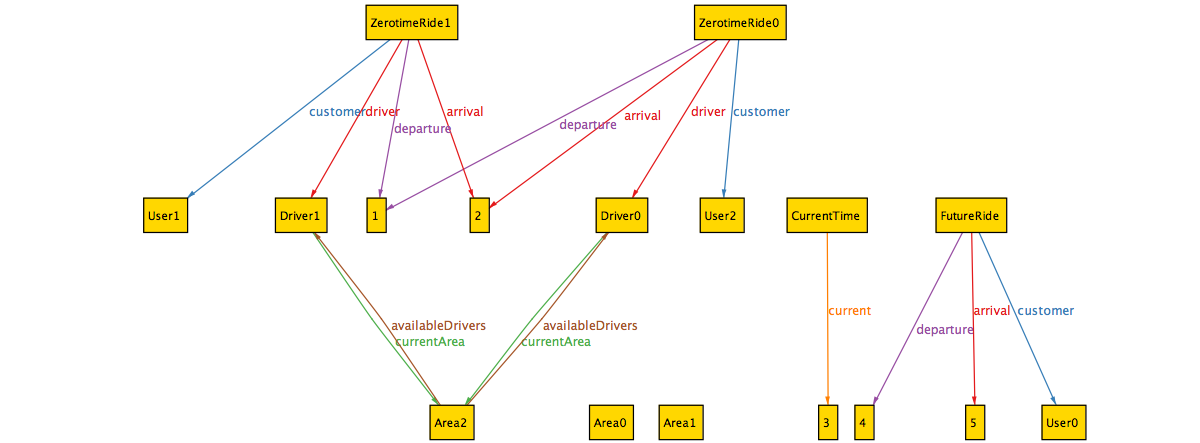
\includegraphics[scale=0.93, angle=90]{./figures/ALLOY_FirstPredicate.png}}
	\caption{World created from the first predicate noDriverAsCustomer}
	\label{w1fig}
\end{figure}

\clearpage

\subsubsection{World 2}
\label{w2}
\begin{figure}[h!]
	\centerline{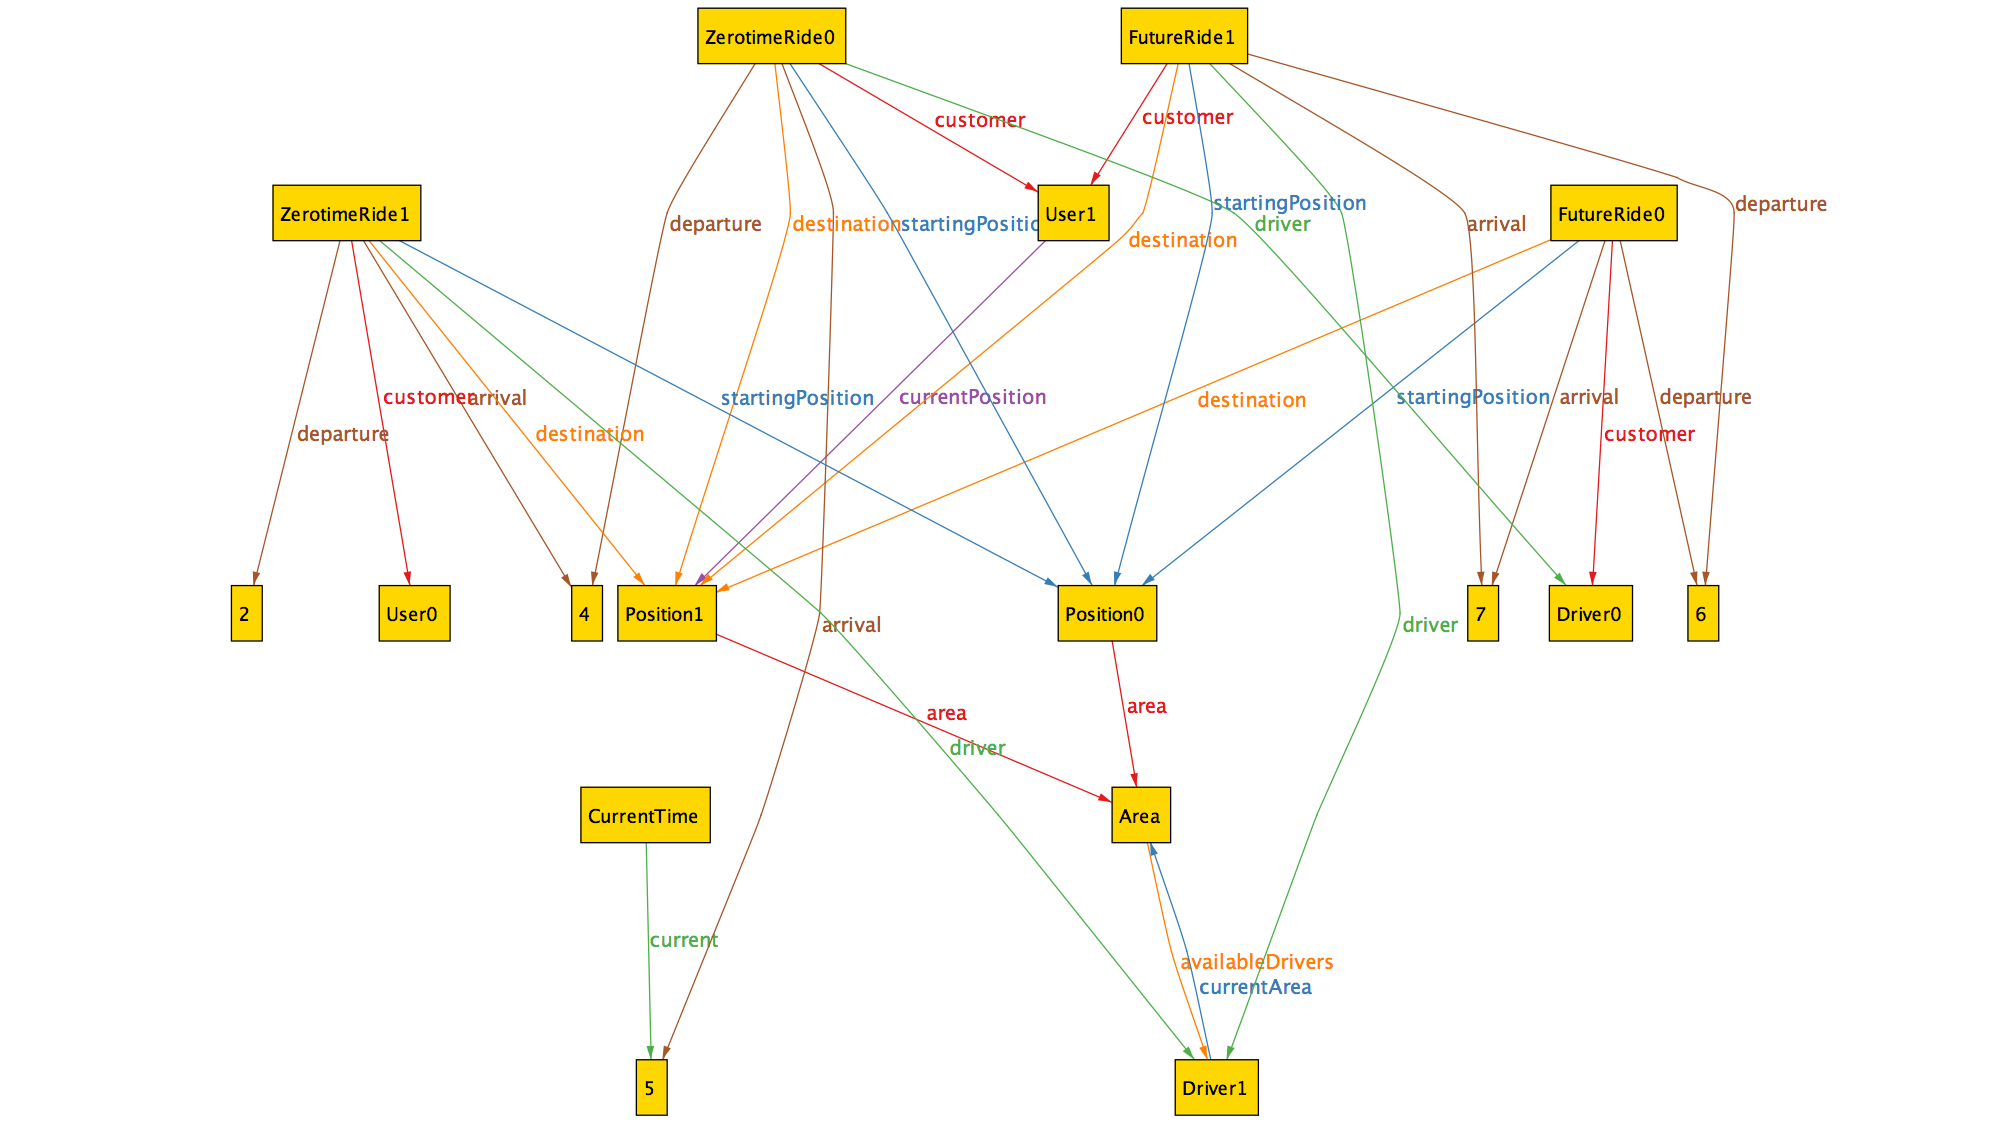
\includegraphics[scale=0.92, angle=90]{./figures/ALLOY_AModelOfTheWorld.png}}
	\caption{World created from the predicate show}
	\label{w2fig}
\end{figure}

%In \figurename~\ref{aw1} is shown the world generated by Alloy Analizer via the execution of the predicate "showInvite". In this predicate the number of users and events is respectively constrained to be greater than 1 and 2. in this way the Analizer generates a significant populated world. It could be assume that the world generated under the imposed constraints is consistent.

%\subsubsection{Word 2}
%\begin{figure}
	%\centerline{\includegraphics[scale=0.9, angle=90]{./Figures/alloyWorld2.png}}
	%\caption{World created from the predicate show}
	\label{aw2}
%\end{figure}

%In \figurename~\ref{aw2} is shown the world generated by Alloy Analizer via the execution of the predicate "show". In this predicate there are no constraints. The predicate generates a world that respects the given constraints where each entities has at maximum 3 instances.

%\subsubsection{World 1 bis}
%\begin{figure}
%	\centerline{\includegraphics[scale=0.5, angle=90]{./Figures/alloyWorld3.png}}
	%\caption{World created from the predicate showInvite with skolemization option enabled}
	\label{aw3}
%\end{figure}

%in \figurename~\ref{aw3} is shown the same world presented in \ref{w1}, but in this case the skolemization option is enabled.

%\section{Alloy Result Evaluation}
%Observing the generated world in \figurename~\ref{aw3}, the existence of some skolemization functions, that are disabled in the model presented in \figurename~\ref{aw1}, can be extrapolated.
%One first conclusion could be simply done from the Alloy code presented. It's likely that some "fact" over the calendar behaviour has inside unnecessary existential quantifiers over the variable "c" (that refers to Calendar). But the need to introduce this quantifiers is directly consequence of the model representation that is been chosen to adopt.
%So it's safe to say that the skolem function are also consequences of the cycles introduced in paragraph concerning the UML Class Diagram. This proves the hypothesis made in the chapter about the data redundancy, showing that the same relation can be obtained without the use of the class Calendar. In spite of that is still useful to regroup connected data and to a simpler visual comprehension,  at least in this first part of the project. During the following project phases the elimination of these redundancies could be taken into account. 

\acresetall